\chapter{Módulos do aplicativo}
\label{apendice_c}
\begin{figure}[!h]
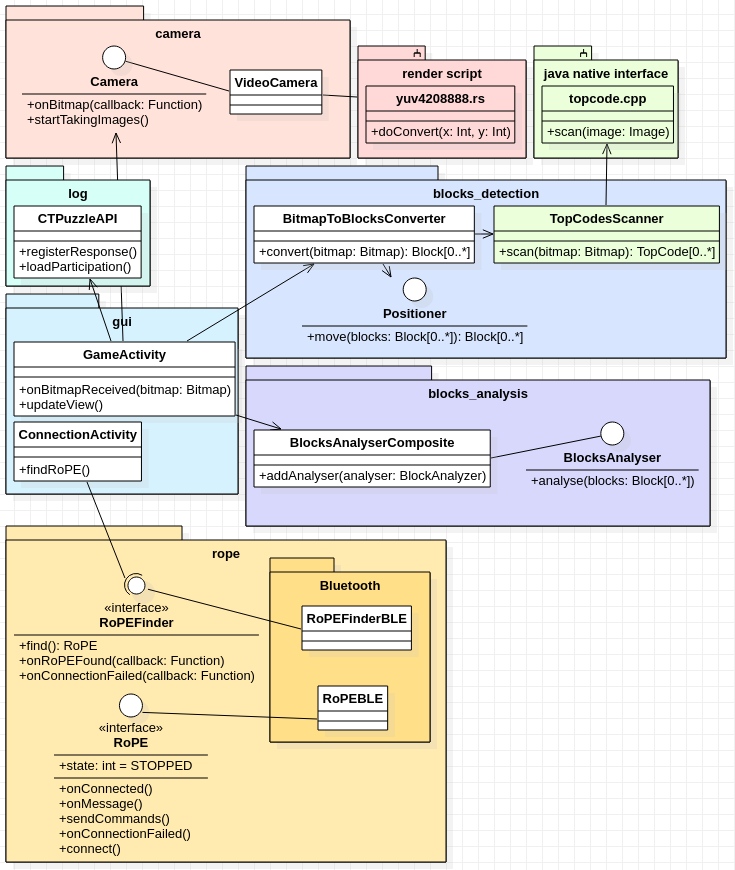
\includegraphics[width=0.9\textwidth,fbox]{figs/app_modules.png}
\caption{Módulos do aplicativo de realidade aumentada.}
\end{figure}

A organização em módulos facilita o reuso do código por trabalhos futuros. Um módulo possivelmente útil é o de comunicação com o RoPE, que abstrai a complexidade de utilização do Bluetooth. Duas tecnologias essenciais para a execução do projeto foram o Render Script e a \textit{Java Native Interface} (JNI). O Render Script foi utilizado para converter imagem produzida pela câmera de formato YUV para RGB, exigido pela biblioteca Topcodes. O JNI permitiu invocar código nativo (escrito em C++), o que diminuiu o tempo de identificação dos topcodes.

Os módulos de detecção de blocos e análise de blocos se diferenciam pelo que o primeiro recebe uma imagem e transforma em objetos tratados pelo aplicativo, como blocos, marcas de calibragem e objeto RoPE. O módulo de análise possui um conjunto de analisadores, que observam o posicionamento desses objetos e emitem eventos. Um exemplo de analisador é o \mintinline{java}{ProgramDetector}, que observa se há uma sequência de blocos encaixados formando um algoritmo e então notifica o controle principal, que envia o algoritmo ao RoPE.
